% ===================================================================
% Arquivo: capitulos/parte-III-pilares/cap-06-retropropagacao-e-gradiente.tex
% ===================================================================

\chapter{O Algoritmo da Repropropagação e Os Otimizadores Baseados em Gradiente}
\label{cap:retropropagacao-gradiente}

% ===================================================================
% Resumo do capítulo
% ===================================================================

% ===================================================================
% Método do Gradiente Descendente
% ===================================================================

\section{O Método do Gradiente Descendente}

O Método do Gradiente faz parte de uma série de métodos numéricos que possuem como função otimizar diferentes funções. Métodos dessa forma veem sendo estudados a séculos, um exemplo disso é o trabalho \textit{M{\'e}thode g{\'e}n{\'e}rale pour la r{\'e}solution des syst{\`e}mes d'{\'e}quations simultan{\'e}es} (Método geral para resolução de sistemas de equações simultâneos em portguês) do matemático francês do século XVIII \textcite{CauchyMetodoDoGradiente}, em que o autor apresenta um método que pode ser considerado um precursor para o método do gradiente atual.

Nesse texto, o autor apresenta uma forma de minimizar uma função de múltiplas variáveis ($u=f(x,y,z)$) que não assume valores negativos, para fazer isso, ele faz uso do cálculo de derivadas parciais dessa função de cada um dos seus componentes ($D_x u, D_y u, D_z u$), em seguida, ele realiza um passo de atualização, de forma que os os valores de cada uma das variáveis sejam ligeiramente incrementados por valores ($\alpha, \beta, \gamma$) \parencite{CauchyMetodoDoGradiente}. Um ponto importante destacado por \textcite{CauchyMetodoDoGradiente} é de que esses incrementos devem ser proporcionais ao negativo das suas respectivas derivadas parciais, ele descreve que esse processo de calcular as derivadas e fazer pequenos incrementos deve ser feito de forma iterativa, assim, calculá-se as derivadas, faz-se os incrementos, e o passo é repetido até convergir para o valor mínimo de $u$.

Esse trabalho explica bem como aplicar o método do gradiente para se calcular mínimos de funções, mas para facilitar o entendimento do leitor, em seguida está um exemplo ilutrativo explicando o funcionamento dessa ferramenta.

\subsection{Exemplo Ilustrativo: Cadeia de Montanhas}

Imagine que você adora aventuras, e por isso, decidiu fazer uma trilha em uma floresta que fica em uma cadeia de montanhas que podem ser escaladas. Então, você teve a incrivel ideia de ir para o menor ponto dessa cadeia de montanhas, pois, no guia que você estava seguindo, falava que lá havia um lago com uma água cristalina, perfeito para tirar fotos.

Para chegar até esse lago, você conta com uma bússula um tanto quanto diferente, ao invés dela apontar para o norte como uma bússola comum, ela aponta para a direção do lugar com menor altitude de uma região. Isso é perfeito para o que você precisa, pois ela irá apontar justamente para o lago de você quer ir.

Com isso em mente, você criou um plano de como irá chegar a esse lago, ele é método que segue dois passos diferentes, sendo eles:

\begin{enumerate}
    \item Olha na bússola qual a direção ela está apontando;
    \item Anda um metro na direção apontada pela bússola.
\end{enumerate}

Você chegou na conclusão que se seguir essa estratégia repetidas vezes, em algum momento, você inevitavelmente irá chegar no lago que está querendo tirar as suas fotos.

Na matemática, existe um método semelhante a este, que busca com base em uma bússola (chamada de vetor gradiente), encontrar um ponto de mínimo de um determinado lugar (neste caso, uma função composta por múltiplas variáveis). Esse é o método do gradiente, ele é ponto central desse capítulo, pois, ele (e suas variações) junto com o algortimo da retroprogação são algumas das principais ferramentas que colaboram para que os modelos de aprendizado de máquina possam aprender com os seus erros e com isso se tornarem melhores a cada iteração.

\subsection{O Método em Si}

A vantagem do método do gradiente é que ele é uma ferramenta matemática, e por isso pode ser representado utilizando notações mais formais e de forma enxuta. As notações utilizadas por Cauchy são diferentes das que são utilizadas hoje em dia, mas o seu significado não muda. Em \textit{Deep Learning}, \textcite{DeepLearningBook} explicam essa ferramenta através da equação \ref{eq:metodo-do-gradiente} que deve ser repetida por múltiplos passos até o modelo convergir, ou seja, encontrar o ponto de mínimo da função estudada.

\begin{equacaodestaque}{Método do Gradiente Descendente}
    x = x_0 - \epsilon \nabla f(x)
    \label{eq:metodo-do-gradiente}
\end{equacaodestaque}

Em que:

\begin{itemize}
    \item $x'$: representa as coordenadas do próximo ponto;
    \item $x$: representa as coordernadas do ponto atual;
    \item $\epsilon$: representa o tamanho do passo, também chamado de taxa de aprendizado;
    \item $\nabla f(x)$: representa o vetor gradiente calculado na posição do ponto atual ($x$) para função que se deseja otimizar.
\end{itemize}

Note que assim como no método proposto por Cauchy, é pego como base o inverso do vetor gradiente. Isso ocorre pois o vetor gradiente é um vetor especial que tem como principal propriedade apontar para a direção de maior crescimento de uma função no ponto que está sendo calculada. Mas no método, o objetivo não é encontrar o ponto que irá gerar os maiores valores da função, e sim o contrário. Por isso, é tomado inverso do vetor gradiente, que, dessa forma, estará então apontando para a direção de menor crescimento de uma função.

Um ponto a ser destacado nesse metodo é na hora de escolher uma taxa de aprendizado para ser utilizada no método. Uma taxa de aprendizado muito pequena signifca que o passo que o modelo irá dar de um ponto para outro será menor, e com isso implica que ele levará mais passos para encontrar um ponto de mínimo. É como se você fosse comparar a quantidade de passos que você gasta para andar do seu quarto até a sua cozinha com a quantidade de passos dados por uma formiga até lá, ambos vão chegar no local, mas a formiga certamente irá demorar bem mais. Considerando isso, surge então a hipótese de que quanto maior for o passo, mais rápido será a convergência, mas isso também não funciona muito bem, pois um passo muito largo pode ultrapassar o ponto de mínimo indo parar em outro canto da função, e ficará tentando chegar até o mínimo mas não irá conseguir pois caminha uma distância muito grande de uma só vez. Essas duas situações, em que o passo é pequeno demais e que o passo e grande demais, são ilustradas na figura \ref{fig:comparativo-tamanho-do-passo}.

\begin{figure}[h!]
    \centering
    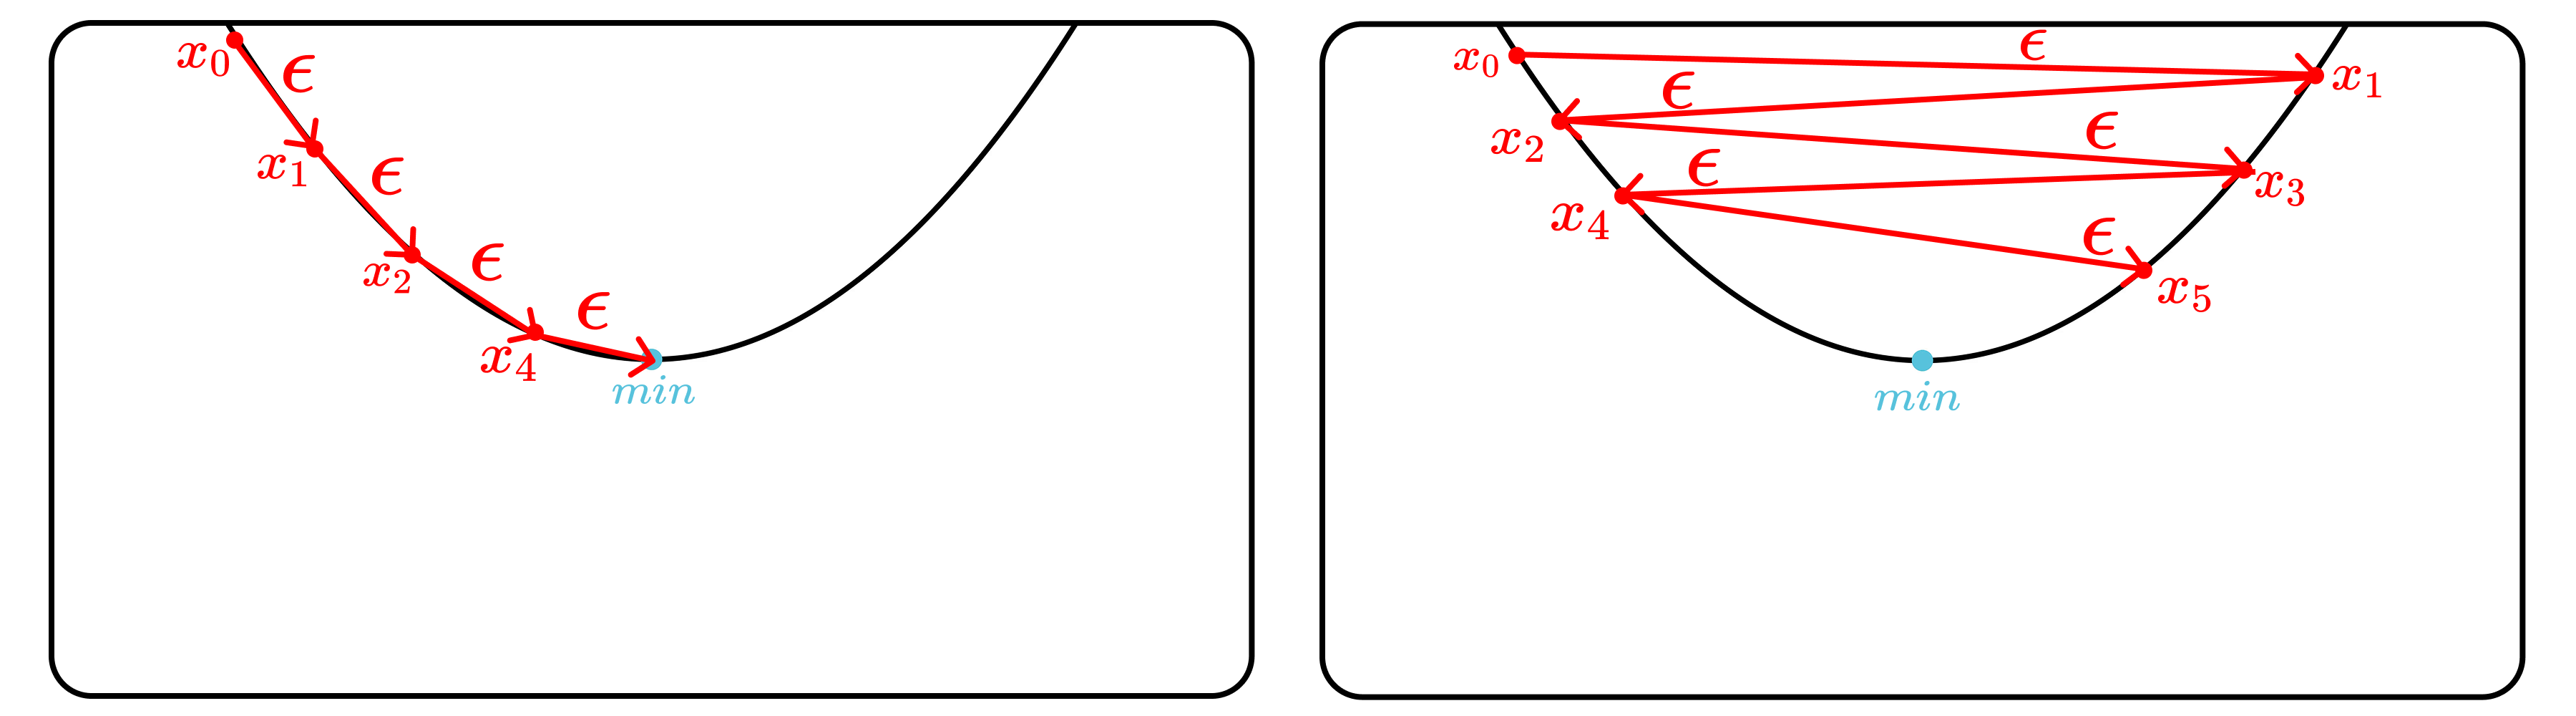
\includegraphics[width=1\linewidth]{../imagens/retropropagacao-gradiente/comparativo-de-passos.png}
    \caption{Comparativo do tamanho de passos em uma função polinomial.}
    \label{fig:comparativo-tamanho-do-passo}
\end{figure}

Na prática, escolher o valor da taxa de aprendizado é uma tarefa que irá depender de modelo em modelo, também irá variar com os diferentes métodos de otimização além da topologia da rede neural que está sendo construída. É sempre recomendado então experimentar diferentes tamanhos de passo, de forma que seja encontrado um que melhor se ajusta ao cenário que está sendo trabalhado.

Outro ponto que deve-se atentar é com relação as funções que estão sendo analisas ao utilizar o método do gradiente mas também qualquer otimizador que seja baseado nele. Se tivermos uma função convexa, em que seu formato lembra um funil, será bem mais fácil para o modelo encontrar o ponto de mínimo global daquela função. Mas se tivermos uma função não convexa, cheia de ondas e com muitos pontos de mínimos locais e pontos de sela, a convergência do modelo será pior, pois existe a chance de que ele fique preso em um ponto de mínimo local ou em um ponto de sela. Isso afeta diretamente o desempenho da rede neural que estará sendo criada, fazendo com que ela tenha métricas piores. O problema é que muitas das vezes a função $f(x)$ que estaremos interessados para calcular o desemepenho do modelo será não convexa, dificultando o seu aprendizado.

Na figura \ref{fig:funcao-convexa-nao-convexa} é possível ver o gráfico de duas funções diferentes, a primeira sendo uma função convexa e a segunda uma função não convexa.

\begin{figure}[h!]
\centering

% --- Gráfico 1: Função 3D Convexa ---
\begin{minipage}{0.48\textwidth}
    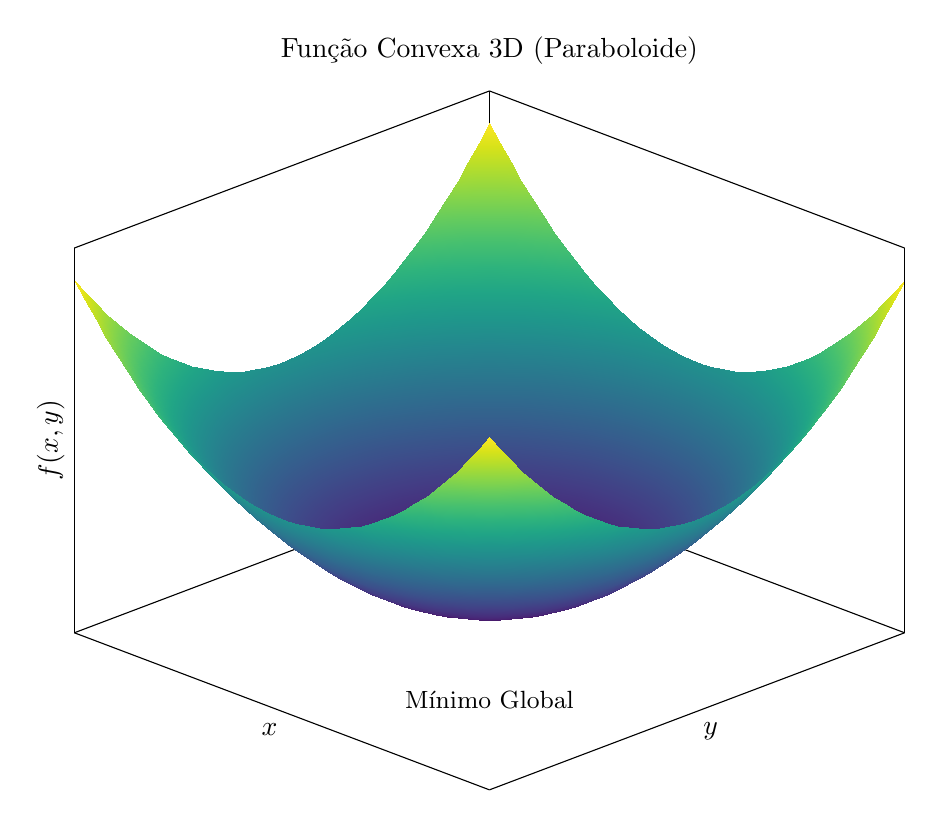
\begin{tikzpicture}
        \begin{axis}[
            title={Função Convexa 3D (Paraboloide)},
            xlabel=$x$,
            ylabel=$y$,
            zlabel={$f(x,y)$},
            xtick=\empty, ytick=\empty, ztick=\empty, % Remove marcações
            view={45}{30}, % Define o ângulo de visão 3D
            width=\textwidth,
            colormap/viridis, % Define o esquema de cores
        ]
        
        % Plot da superfície 3D z = x^2 + y^2
        \addplot3[
            surf, % Tipo de gráfico: superfície
            shader=interp, % Cores interpoladas para um visual suave
            domain=-2:2,
            domain y=-2:2,
            samples=40, % "Resolução" da malha
        ] {x^2 + y^2};
        
        % Marcador para o mínimo global
        \node at (axis cs:0,0,-2) [below, font=\small] {Mínimo Global};
        
        \end{axis}
        \label{fig:funcao-convexa}
    \end{tikzpicture}
\end{minipage}
\hfill % Espaço entre as figuras
% --- Gráfico 2: Função 3D Não-Convexa ---
\begin{minipage}{0.48\textwidth}
    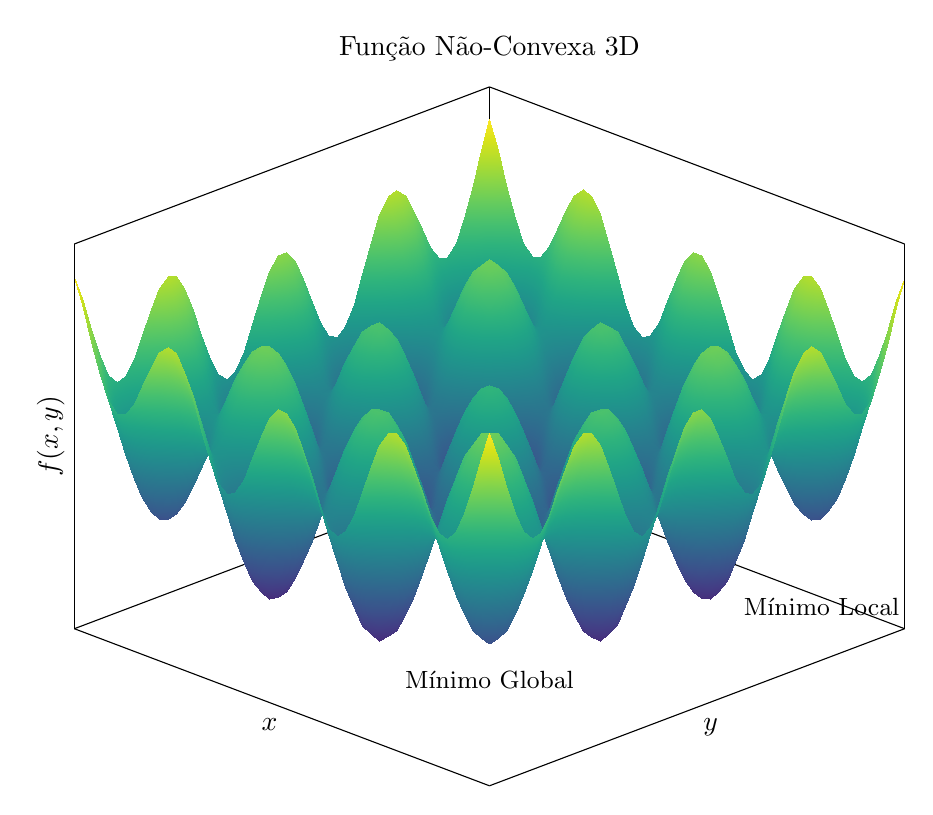
\begin{tikzpicture}
        \begin{axis}[
            title={Função Não-Convexa 3D},
            xlabel=$x$,
            ylabel=$y$,
            zlabel={$f(x,y)$},
            xtick=\empty, ytick=\empty, ztick=\empty,
            view={45}{30},
            width=\textwidth,
            colormap/viridis,
        ]
        
        % Plot da superfície com "ondinhas"
        % A função é um paraboloide + cossenos para criar as ondas
        \addplot3[
            surf,
            shader=interp,
            domain=-2.5:2.5,
            domain y=-2.5:2.5,
            samples=50,
        ] {(x^2+y^2)/5 + 2 - cos(deg(180*x)) - cos(deg(180*y))};
        
        % Marcadores para os mínimos
        \node at (axis cs:0,0,-1) [below, font=\small] {Mínimo Global};
        \node at (axis cs:2,2,0) [font=\small] {Mínimo Local};
        
        \end{axis}
        \label{fig-funcao-nao-convexa}
    \end{tikzpicture}
\end{minipage}
\caption{Comparação entre funções 3D convexas e não-convexas.}
\label{fig:funcao-convexa-nao-convexa}
\end{figure}

\subsection{Implementação em Python}

\begin{algorithm}[H]
\caption{O Método do Gradiente (Descida do Gradiente)}
\label{alg:gradient_descent}
\begin{algorithmic}[1]
\Require Taxa de aprendizado global $\epsilon$
\Require Parâmetros iniciais $\boldsymbol{\theta}$

\State Inicialize os parâmetros $\boldsymbol{\theta}$

\While{critério de parada não for atingido}
    \State Calcule o gradiente $\mathbf{g} \gets \nabla_{\boldsymbol{\theta}} L(\boldsymbol{\theta})$, usando \textbf{todo} o conjunto de treinamento
    \State Calcule a atualização: $\Delta \boldsymbol{\theta} \gets -\epsilon \mathbf{g}$
    \State Aplique a atualização: $\boldsymbol{\theta} \gets \boldsymbol{\theta} + \Delta \boldsymbol{\theta}$
\EndWhile
\end{algorithmic}
\end{algorithm}

Para implementar o método do gradiente utilizando Python e a biblioteca de cálculos Numpy, deve-se seguir como base a equação \ref{eq:metodo-do-gradiente}, criando uma classe implenta essa ferramenta, recebendo como parâmetros de entrada a taxa de aprendizado (\texttt{learning\_rate}), a função que se quer encontrar o ponto de mínimo (\texttt{function}), e um ponto inicial (\texttt{initial\_point}), que pode ser um conjunto de coordenadas aleatórias ou escolhidas pelo programador.

Outro ponto que deve ser destacado nas informações dessa função é de que ela também irá receber a derivada da função (\texttt{function\_prime}) que se quer descobrir o ponto de mínimo, pois não será feito cálculo simbólico para calcular o vetor gradiente. Dessa forma os cálculos serão mais rápidos. Além disso, também é preciso definir outros parâmetros auxiliares, como a quantidade máxima de iterações que o modelo irá seguir (\texttt{tolerance}), que são chamadas de épocas \texttt{epochs}, também será definida um grau de tolerância para o modelo, pois, podem existir casos em que a norma do vetor gradiente são será exatemente zero, mas um valor muito próximo de zero, assim a tolerância será responsável por definir qual valor dessa diferença será aceitável para o problema.

Por fim, um ponto interessante que é possível adicionar nessa função é uma lista, que irá armazenar todos os pontos que o modelo passou em cada uma de suas iterações, indicando o seu caminho pela função que está sendo estudada.

\begin{codelisting}{Classe completa do otimizador GradientDescent}{gd_class}
class GradientDescent:

    def __init__(self, function, function_prime, initial_point, learning_rate=0.001, epochs=100, tolerance=1e-6):
        self.f = function
        self.fp = function_prime
        self.ip = initial_point
        self.lr = learning_rate
        self.ep = epochs
        self.tol = tolerance
        self.path = []

    def update_step(self):
        for i in range(self.ep):
            self.path.append(self.ip)
            grad = self.fp(self.ip)
            if abs(grad) < self.tol: break
            self.ip = self.ip + self.lr * (-grad)
        return self.ip, self.path
\end{codelisting}

Note que a classe apresenta apenas dois métodos, o primeiro sendo o \texttt{\_\_init\_\_}, que inicializa os parâmetros da classe, e a \texttt{update\_step} a qual é responsável por implementar de fato o método do gradiente, ela irá retornar o ponto de mínimo e também a lista com os pontos pelos quais o modelo passou ao longo das iterações.

% ===================================================================
% A Retropropagação
% ===================================================================

\section{A Retropropagação: Aprendendo com os Erros}

Ainda no contexto de utilizar com o vetor gradiente para otimizar um modelo de rede neural, existe uma ferramenta que trabalha justamente com essse processo, ela é a retropropagação ou \textit{backpropagation} em inglês.

\begin{definicaomoderna}{\textbf{Definição:}}
A \textbf{retropropagação} é uma ferramenta que veio para permitir que redes que fazem o uso de unidades de neurônios possam aprender, para isso, o procedimento ajusta repetidamente os pesos das conexões da rede para minimizar a diferença entre o valor atual da saída do vetor da rede neural com o valor real desejado \parencite{BackpropagationArticle}.
\end{definicaomoderna}

Essa ferramenta foi introduzida para a comunidade científica pelos pesquisadores \textcite{BackpropagationArticle} no texto \textit{Learning Representations by Back-Propagating Errors}, e será explicada nesse capítulo de forma detalhada. Para issom \textcite{BackpropagationArticle} comecam introduzindo três diferentes funções que serão utilizadas ao longo do texto para deduzir o os conceitos da retropropagação do gradiente, sendo elas: a equação do neurônio, a função de ativação sigmoide e a função de custo do erro quadrático médio.

A primeira função, representada na equação xx, explica como um neurônio de uma camada densa irá funcionar quando recebe determinadas entradas.

\begin{equacaodestaque}{Equação do Neurônio}
    x_j = (\sum_i y_i \cdot w_{ji}) + b_j
    \label{eq:neuronio-camada-densa}
\end{equacaodestaque}

Sendo que:

\begin{itemize}
    \item $x_j$: representa a saída de um neurônio $j$;
    \item $y_i$: representa a entrada do neurônio $j$, a qual é resultado da saída de um neurônio $i$ da camada anterior;
    \item $w_{ij}$: representa o peso da conexão entre o neurônio $i$ com o neurônio $j$;
    \item $b_j$: representa o viés do neurônio $j$.
\end{itemize}

Caso você leitor decida olhar o artigo original, verá que os autores utilizaram notações diferentes na fórmula do neurônio, eles utilizam algo na forma $x_i = \sum_i y_i \cdot w_{ji}$, sem o viés, mas na prática, eles adicionam o viés como um peso extra que terá valor fixo igual a 1, na prática, ele pode ser tratado com um peso normal, por isso a notação mais simplificada \parencite{BackpropagationArticle}.

A segunda fórmula diz respeito a função de ativação que será utilizada, neste caso, \textcite{BackpropagationArticle} utilizam a sigmoide logísitca, representada na fórmula xx, mas eles explicam que essa função pode variar conforme o problema, porém recomendam ter uma derivada limitada além de ser não linear, para que o modelo possa aprender de forma mais efciente.

\begin{equacaodestaque}{Sigmoide Logística}
    y_j = \sigma(x_j) = \frac{1}{1 + e^{-x_j}}
    \label{eq:sigmoide}
\end{equacaodestaque}

Assim, a sigmoide é a função que irá transformar a saída do neurônio $x_j$ em uma saída $y_j$ que vai ser passada para o neurônio da camada seguinte. Além das duas notações da equação do neurônio, existe uma terceira, que já imbute a função de ativação na equação do neurônio, nesse livro, utilizaremos uma implementação de camadas, em que elas não possuem a função embutida, assim, caso decida que a saída da camada densa deva passar por uma função de ativação, ela deverá ser passada como uma camada separada, sendo algo da forma: camada densa, seguida de camada de ativação.

Por fim, a última equação que os autores discutem para entender a retropropagação é a da função de custo, ou também chamada de erro. No texto, \textcite{BackpropagationArticle} utilizam a função do erro quadrático médio (MSE), a qual calcula o erro entre a saída atual do modelo e o valor real desejado, depois ela eleva ao quadrado esse valor, e por último, divide por dois. Ela é dada pela equação:

\begin{equacaodestaque}{Erro Quadrático Médio (MSE)}
    E = \frac{1}{2} \sum_{c} \sum_{j} (y_{j, c} - d_{j, c})^2 
    \label{eq:mse}
\end{equacaodestaque}

Em que:

\begin{itemize}
    \item $E$: representa o valor do erro;
    \item $y_{j, c}$: representa o valor atual da saída do neurônio $j$ para o caso $c$;
    \item $d_{j, c}$: representa o valor desejado para o neurônio $j$ para o caso $c$
\end{itemize}

Considerando essas equações, \textcite{BackpropagationArticle} explicam que o objetivo é reduzir o valor do erro $E$, para isso, eles aplicam o método do gradiente para encontrar o ponto de mínimo da função MSE. Para isso, o primeiro passo é diferenciar o valor da função de erro em relação a cada um dos pesos da rede neural, assim, deve-se calcular $\partial E / \partial y_k$ para um caso específico $k$, e depois generalizar a situação. Assim, é possível encontrar uma expressão da forma:

\[
    \frac{\partial E}{\partial y_k} = \frac{\partial}{\partial y_k} \left[ \frac{1}{2} \sum_c \sum_k (y_{k, c} - d_{j, c})^2\right]
\]

O primeiro passo é suprimir a soma sobre os casos $c$, pois, consideramos apenas de um caso específico $k$, então a expressão se simplifica para:

\[
    \frac{\partial E}{\partial y_k} = \frac{\partial}{\partial y_k} \left[ \frac{1}{2} \sum_k (y_{k, c} - d_{j, c})^2\right]
\]

O próximo passo é abrir a soma, para isso, será considerado que existem $n$ neurônios na camada, assim, a expressão fica:

\[
    \frac{\partial E}{\partial y_k} = \frac{\partial}{\partial y_k} \left[ \frac{1}{2} \left( (y_1 - d_1)^2 + (y_2 - d_2)^2 + \cdots (y_k + d_k)^2 + \cdots + (y_n + d_n)^2 \right) \right]
\]

Note que todos os termos que não possuem o índice $k$, como a parte $(y_1 - d_1)^2$, serão valores constantes, e que estarão fora do obejtivo de calcular a derivada para o neurônio $k$, como eles são constantes, a sua derivada será igual a zero. Com base nisso, é possível obter uma versão ainda mais simplificada, sendo ela:

\[
    \frac{\partial E}{\partial y_k} = \frac{\partial}{\partial y_k} \left[ \frac{1}{2} (y_k + d_k)^2 \right]
\]

Agora, o último passo é aplicar a regra da cadeia na expressão que sobrou para poder calcular a derivada, neste caso, será considerado que $u = (y_k + d_k)$, assim a expressão final fica:

\[
    \frac{\partial E}{\partial y_k} = \frac{1}{2} \cdot 2u \cdot \frac{\partial u}{\partial y_k} = (y_k - d_k) \cdot 1 = (y_k - d_k)
\]

Voltando para o índice $j$ da notação inicial, é possível concluir que o gradiente do erro (para a função MSE) em relação a uma saída específica de um neurônio é dado pela diferença da saída da unidade pela resultado desejado, ou seja

\[
    \frac{\partial E}{\partial y_j} = (y_j - d_j) 
\]

O próximo passo proposto pelos autores, consiste em calcular o gradiente do erro em relação a entrada do neurônio $j$, para entender como o erro total muda em relação a uma variação na entrada do neurônio. Para isso, é preciso encontrar então a expressão $\partial E / \partial x_j$ \parencite{BackpropagationArticle}.

Assim, a primeira etepa é aplicar a regra da cadeia, pois, como a entrada do neurônio $x_j$ não aparece diretamente na equação do erro, é preciso aplicar a regra da cadeia, derivando o erro em relação a saída do neurônio $y_j$ e multiplicando esse resultado pela derivada da saída do neurônio em relação a sua entrada, assim, a expressão inicial é:

\[
    \frac{\partial E}{\partial x_j} = \frac{\partial E}{\partial y_j} \cdot \frac{\partial y_j}{\partial x_j}
\]

Perceba duas coisas nessa expressão, a primeira é que o primeiro termo é resultamente o primeiro que foi calculado e desenvolvido na expressão \ref{eq:gradiente-do-erro-em-relacao-a-saida-de-um-neuronio}, com isso, é possível substituir esse termo na expressão por $y_j - d_j$. A segunda informação, é de que o termo $\partial y_i / \partial x_j$ é justamente a derivada da função de ativação em relação a sua entrada, ou seja, $\sigma'(x_j)$, assim, a derivada da sigmoide será dada por:

\[
    \frac{d y_i}{d x_j} = y_j (1 - y_j)
\]

Sendo assim, a expressão final fica:

\[
    \frac{\partial E}{\partial x_j} = \frac{\partial E}{\partial y_j} \cdot y_j \cdot (1 - y_j)
\]

Note que é possível generalizar essa expressão, dessa forma o gradiente do erro da entrada de um neurônio é o gradiente do erro da saída do neurônio multiplicado pela derivada da função de ativação $\sigma'$ em relação a sua entrada $x_j$.

\begin{equacaodestaque}{Cálculo do Gradiente do Erro em Relação à Entrada de um Neurônio}
    \frac{\partial E}{\partial x_j} = \frac{\partial E}{\partial y_j} \cdot \sigma'(x_j)
    \label{eq:gradiente-do-erro-em-relacao-a-entrada-de-um-neuronio}
\end{equacaodestaque}

em que $\sigma'(x_j)$ representa a derivada de uma função de ativação qualquer, neste caso representa a sigmoide logística. Mas pode ser outra função, como a tangente hiperbólica ou a ReLU. Um ponto importante a ser destacado, é que como a retropropagação trabalha com o método do gradiente, as derivadas são parte essencial do algoritmo, utilizar funções de ativação que possuem derivadas complexas, ou que não podem ser derivadas em grande parte do seu domínio, acabam por difultar o algortimo. Caso a função possua uma derivada complexa, o cálculo do gradiente irá demorar mais, pois levará uma quantidade maior de operações para computar o valor da derivada.

O próximo passo vai mais além ainda, agora, como \textcite{BackpropagationArticle} explicam, o seu objetivo é entender como o gradiente muda em relação a um peso $w_ij$ específico da rede neural, para isso, é preciso calcular a expressão $\partial E / \partial w_{ij}$, note mais uma vez que o peso $w_{ij}$ não aparece diretamente na equação do erro, assim, é necessário mais uma vez aplicar a regra da cadeia para calcular essa derivada. Assim, a expressão inicial é:

\[
    \frac{\partial E}{\partial w_{ij}} = \frac{\partial E}{\partial x_j} \cdot \frac{\partial x_j}{\partial w_{ij}}
\]

Note que o primeiro termo da expressão é justamente o que foi calculado na equação \ref{eq:gradiente-do-erro-em-relacao-a-entrada-de-um-neuronio}, assim, é preciso calcular apenas o segundo termo, $\partial x_i / \partial w_{ij}$, ou seja, a derivada do neurônio em relação a um peso específico. Assim, tem-se a expressão incial:

\[
    \frac{\partial x_j}{\partial w_{ij}} = \frac{\partial}{\partial w_{ij}} \left[ \left( \sum_i y_i \cdot w_{ji} \right) + b_j\right]
\]

Note que o viés, dado por $b_j$ é uma constante, e por isso, não depende do peso $w_{ij}$, então a sua derivada será igual a zero, isso nos permite simplicar a expressão para:

\[
    \frac{\partial x_j}{\partial w_{ij}} = \frac{\partial}{\partial w_{ij}} \left[\sum_i y_i \cdot w_{ji}\right]
\]

Em seguida, é possível abrir a soma, assim, temos a expressão:

\[
    \frac{\partial x_j}{\partial w_{ij}} = \frac{\partial}{\partial w_{ij}} \left[ (y_1 \cdot w_{j1}) + (y_2 \cdot w_{j2}) + \cdots (y_i \cdot w_{ji}) + \cdots (y_n \cdot w_{jn})\right]
\]

Note que para qualquer termo que o índice não é $w_{ji}$ a derivada será iguala zero, pois eles serão constantes em relação ao peso $w_{ji}$, dessa forma, é possível simplificar mais uma vez a expressão obtendo:


\[
    \frac{\partial x_j}{\partial w_{ij}} = \frac{\partial}{\partial w_{ij}} \left[  y_i \cdot w_{ji} \right]
\]

Como $y_i$ é uma constante em relação a $w_ij$ a derivada final será dada por:

\[
    \frac{\partial x_j}{partial w_{ij}} = y_i
\]

Agora é possível voltar para a expressão inicial, obtendo então a expressão final para o gradiente do erro em relação a um peso específico da rede neural, sendo ela:

\begin{equacaodestaque}{Cálculo do Gradiente do Erro em Relação a um Peso de um Neurônio}
    \frac{\partial E}{\partial w_{ij}} = \frac{\partial E}{\partial x_j} \cdot y_i = \frac{\partial E}{\partial y_j} \cdot \sigma'(x_j) \cdot y_i
    \label{eq:gradiente-do-erro-em-relacao-a-um-peso-de-um-neuronio}
\end{equacaodestaque}

Assim, é possível concluir que o gradiente do erro em relação a um peso específico de um neurônio é dado pelo gradiente do erro da saída do neurônio multiplicado pela derivada da função de ativação em relação a sua entrada e, por fim, multiplicado pela entrada do neurônio.

O próximo passo não está no artigo original, ele envolve entender como o erro varia em relação a um viés de um neurônio específico, ou seja, é preciso calcular a expressão $\partial E / \partial b_j$. Note que mais uma vez o viés $b_j$ não aparece diretamente na equação do erro, ele está dentro da equação do neurônio, assim, novamente é preciso aplicar a regra da cadeia para encontrar essa derivada, assim, a expressão inicial é dada por:

\[
    \frac{\partial E}{\partial b_j} = \frac{\partial E}{\partial x_j} \cdot \frac{\partial x_j}{\partial b_j}
\]

A primeira expressão, $\partial E / \partial x_j$, já foi calculada na equação \ref{eq:gradiente-do-erro-em-relacao-a-entrada-de-um-neuronio}, assim, é preciso focar apenas na segunda parte da expressão, $\partial x_j / \partial b_j$, que avalia como a saída do neurônio $x_j$ varia em relação ao viés $b_j$. Com base, nisso, é possível chegar na expressão:

\[
    \frac{\partial E}{\partial b_j} = \frac{\partial}{\partial b_j} \left[ \left( \sum_k y_k \cdot w{jk} \right) + b_j \right]
\]

Note que os termos que não possuem o viés, como a parte que faz a soma da multiplicação das entradas pelos pesos, $\sum_l y_k \cdot w_{jk}$, são constantes em relação ao viés, portanto, a sua derivada será igual a zero, de tal forma que é possível simplificar a expressão para:

\[
        \frac{\partial E}{\partial b_j} = \frac{\partial}{\partial b_j} \left[ b_j \right]
\]

Com base nessa expressão, é possível concluir que a derivada da saída do neurônio em relação ao viés é igual a 1. Assim, voltando para a expressão inicial, temos que o gradiente do erro em relação ao viés de um neurônio específico é dado pelo gradiente do erro da entrada entrada total desse neurônio, ou seja:

\begin{equacaodestaque}{Cálculo do Gradiente do Erro em Relação a um Viés de um Neurônio}
    \frac{\partial E}{\partial b_j} = \frac{\partial E}{\partial x_j} \cdot 1 = \frac{\partial E}{\partial y_j} \cdot \sigma'(x_j)
    \label{eq:gradiente-do-erro-em-relacao-a-um-vies-de-um-neuronio}
\end{equacaodestaque}

\subsection{Utilizando o Gradiente Descendente para Atualizar os Pesos e Vieses}

Já que é possível calcular o gradiente do erro em relação a um peso específico de um neurônio, e também em relação a um viés específico de um neurônio, o próximo passo proposto pelos autores é utilizar o método do gradiente como uma forma de atualizar os pesos (e também os vieses no nosso caso) da rede neural, de forma a minimizar o valor do erro com pequenas atualizações em cada um desses parâmetros \parencite{BackpropagationArticle}.

Note que o método do gradiente, explicado na seção anterior diz que para atualizar um parâmetros, é preciso pegar o valor atual do parâmetro, e subtrair dele o valor do gradiente multiplicado pelo tamanho do passo (ou taxa de aprendizado). dessa forma, a regra de atualização para um peso específico é dada pela equação \ref{eq:regra-de-atualizacao-de-um-peso-atraves-do-metodo-do-gradiente}


\begin{equacaodestaque}{Regra de Atualização de um Peso Através do Método do Gradiente}
    w_{t+1} = w_{t} - \epsilon \frac{\partial E}{\partial w}
    \label{eq:regra-de-atualizacao-de-um-peso-atraves-do-metodo-do-gradiente}
\end{equacaodestaque}

Em que:

\begin{itemize}
    \item $w_{t+1}$ representa o valor do peso atualizado após o incremento do método do gradiente;
    \item $w_t$ representa o valor inicial do peso na iteração $t$;
    \item $\epsilon$ representa o tamanho do passo / taxa de aprendizado;
    \item $\partial E / \partial w$ representa o gradiente do erro em relação ao peso.
\end{itemize}

Analogamente, a regra de atualização de um viés pelo método do gradiente é dada pela equação \ref{eq:regra-de-atualizacao-de-um-vies-atraves-do-metodo-do-gradiente}

\begin{equacaodestaque}{Regra de Atualização de um Viés Através do Método do Gradiente}
    b_{j, t+1} = b_{j, t} - \epsilon \frac{\partial E}{\partial b_j}
    \label{eq:regra-de-atualizacao-de-um-vies-atraves-do-metodo-do-gradiente}
\end{equacaodestaque}

Neste caso, $b_{j, t+1}$ representa o valor final de um viés $j$ após o incremento do método e $b_{j, t}$ o valor inicial do viés $j$.

Um ponto a ser destacado, é que quando estiver trabalhando com uma camada densa de neurônios, você não irá lidar com um neurônio específico, e sim como uma conjunto inteiro deles. Dessa forma, eles estrão distribuidos de forma vetorizada, que que terá um vetor de viéses, uma matriz de pesos e um vetor de neurônios. Assim, as expressões {eq:regra-de-atualizacao-do-vetor-de-pesos-atraves-do-metodo-do-gradiente} e \ref{eq:regra-de-atualizacao-do-vetor-de-vieses-atraves-do-metodo-do-gradiente}, resumem as regras de atualização de pesos e vieses, respectivamente, para casos em que estiver lidando com um conjunto de vetores ao invés de somente um dado.

\begin{equacaodestaque}{Regra de Atualização do Vetor de Pesos Através do Método do Gradiente}
    \mathbf{w}_{t+1} = \mathbf{w}_t - \epsilon \nabla_{\mathbf{w}} E
    \label{eq:regra-de-atualizacao-do-vetor-de-pesos-atraves-do-metodo-do-gradiente}
\end{equacaodestaque}

\begin{equacaodestaque}{Regra de Atualização do Vetor de Vieses Através do Método do Gradiente}
    \mathbf{b}_{t+1} = \mathbf{b}_t - \epsilon \nabla_{\mathbf{b}} E
    \label{eq:regra-de-atualizacao-do-vetor-de-vieses-atraves-do-metodo-do-gradiente}
\end{equacaodestaque}

\subsection{Entendendo Como o Gradiente É Propagado ao Longo de Muitas Camadas}

Por fim, com base no que foi explicado até agora, é possível entender melhor como o gradiente passa de uma acamada para a outra durante a retropropagação, para isso será analisada um rede com quatro camadas densas, sendo elas:

\begin{itemize}
    \item \textbf{Camada 1 (Entrada):}: Ela possui neurônios com o indice $i$;
    \item \textbf{Camada 2 (Oculta 1):}: Ela possui neurônios com o indice $j$;
    \item \textbf{Camada 3 (Oculta 3):}: Ela possui neurônios com o indice $k$;
    \item \textbf{Camada 4 (Oculta 3):}: Ela possui neurônios com o indice $l$;
\end{itemize}

O objetivo é calcular o gradiente de um peso da primeira camada de pesos, $w_{ji}$, ou seja, é um peso que conecta um neurônio da camada $i$ com um neurônio da camada $j$. Assim, o primeiro passo é utilizar a fórmula \ref{eq:gradiente-do-erro-em-relacao-a-um-peso-de-um-neuronio}, que calcula o gradiente do erro em relação a um peso quaquer.

\[
    \frac{\partial E}{\partial w_{ij}} = \frac{\partial E}{\partial x_j} \cdot y_i
\]

Para encontrar esse gradiente, é preciso desenvolver a expressão $\partial E / \partial x_j$, que representa o gradiente do erro da entrada de um neurônio $j$ da primeira camada oculta. Para isso, é possível utilizar como base a equação \ref{eq:gradiente-do-erro-em-relacao-a-entrada-de-um-neuronio}, obtendo então:

\[
    \frac{\partial E}{\partial x_j} = \frac{\partial E}{\partial y_j} \cdot \sigma'(x_j)
\]

Nessa expressão, $\sigma'(x_j)$ representa a função de ativação, já o termo $\partial E / \partial y_j$ representa o gradiente que está vindo ca camada de cima, o qual é dado por:

\[
    \frac{\partial E}{\partial x_j} = \sum_k \frac{\partial E}{\partial x_k} \cdot w_{kj}
\]

Juntando os dois termos:

\[
    \frac{\partial E}{\partial x_j} = \left( \sum_k \frac{\partial E}{\partial x_k} \cdot w_{kj} \right) \sigma'(x_j)
\]

Agora, é preciso calcular o termo $\partial E / \partial x_j$, de forma que será possível trazer o gradiente da camada de saída $l$, assim temos:

\[
    \frac{\partial E}{\partial x_k} = \left( \sum_k \frac{\partial E}{\partial x_l} \cdot w_{lk} \right) \cdot \sigma'(x_k)
\]

Em que $\partial E / \partial x_l$ representa o primeiro gradiente, ele é calculado na camada de saída.

Por último, é preciso combinar essas expressões, encontrando como resultado a expressão:

\[
    \frac{\partial E}{\partial w_{ij}} = \left( \sum_k \left[ \left( \sum_l \frac{\partial E}{\partial x_l} \cdot w_{lk} \right) \sigma'(x_k) \right] \cdot w_{kj} \right) \sigma(x_j) \cdot y_i
\]

Com base nessa expressão, é possível concluir que o gradiente de uma camada inicial é proporcional a uma cadeia de multiplicações dos pesos e das derivadas das funções de ativação das camadas posteriores, de forma que é possível simplificar isso para:

\[
    \frac{\partial E}{\partial w_{\text{primeira camada}}} \propto (\text{gradiente da saída}) \cdot (w_{\text{camada 3}} \cdot \sigma'_{\text{camada 3}}) \cdot (w_{\text{camada 2}} \cdot \sigma'_{\text{camada 2}})
\]

Generalizando essa expressão, é possível concluir que o gradiente para uma camada é dado ela equação \ref{eq:gradiente-para-n-camadas}.

\begin{equacaodestaque}{Gradiente para N Camadas}
    \delta^{(L)} = \left( \left( \textbf{W}^{(L+1)} \right)^T \delta^{(L+1)} \right)  \odot \sigma'(x^{(L)})
    \label{eq:gradiente-para-n-camadas}
\end{equacaodestaque}

Em que: 

\begin{itemize}
    \item $L$: Representa o índice de uma camada, podendo ser um valor entre $1$ (indicando que é uma camada de entrada) ou $n$ (indicando que é uma camada de saída);
    \item $\textbf{W}^{(L)}$: Representa a matriz dde pesos que conecta a camada $L - 1$ à camada $L$;
    \item $b^{(L)}$: Representa o vetor de viés da camada $L$;
    \item $x^{(L)}$: Representa o vetor de entradas totais para os neurônios da camada $L$ antes da ativação;
    \item $y^{(L)}$: Representa o vetor de saídas da camada $L$
    \item $\delta^{(L)}$: Representa o vetor do gradienye na camada $L$;
    \item $\sigma'(x^{(L)})$: Representa o vetor contendo a derivada da função de ativação para cada neurônio da camada $L$;
    \item $\odot$: O produto de Hadamard, que significa multiplicação elemento a elemento.
\end{itemize}

Assim, é possível entender como o gradiente irá se propagar ao longo de uma rede neural. Esse ponto é um dos mais importantes, pois é possível considerar que ele terá uma grande relação com as funções de ativação que são utilizadas. Essa é uma relação complicada, pois, enquanto um determinado tipo de função possa causar um tipo de problema no cálculo do gradiente, e por isso não deve ser uma opção viável para ser escolhida para resolver um problema, optar por outra família de função também pode acarretar outro tipo de problema com o gradiente.

Para isso, o capítulo \ref{cap:ativacao-sigmoidais} foca em entender as pricipais funções sigmoidais, como a sigmoide e a tangente hiperbólica, e como essas possuem uma forte relação com o problema do desaparecimento de gradientes. Em seguida, o capítulo \ref{cap:ativacao-retificadoras} busca introduzir as funções retificadoras, como a ReLU, e como elas podem ser uma alternativa para contornar esse problema. Contudo, isso não as torna perfeitas, elas ainda são suceptíveis à outro tipo de problema: a explosão de gradientes; e, no caso da ReLU: o problema dos neurônios agonizantes.

% ===================================================================
% Otimizadores Baseados em Gradiente
% ===================================================================

\section{Otimizadores Baseados em Gradiente}

Como \textcite{BackpropagationArticle} explicam logo ao terminar a dedução do cálculo da atualização dos pesos utilizando o método do gradiente, esse processo pode ser bastante lento quando comparado com métodos que fazem uso de derivadas de segunda ordem, que certamente são mais caras para serem implementadas no computador. Assim, os autores recomendam uma variação do método do gradiente que faz uso de momentum com intuito de acelerar a convergência a um custo computacional menor que o de implementar derivadas de segunda ordem \parencite{BackpropagationArticle}.

\subsection{Método do Gradiente com Momentum}

\subsubsection{Implementação em Python}

\subsection{Método do Gradiente Estocástico}

\subsubsection{Implementação em Python}

\section{Otimizadores Modernos Baseados em Gradiente}

\subsection{Nesterov}

\subsubsection{Implementação em Python}

\subsection{AdaGrad}

\subsubsection{Implementação em Python}

\subsection{RMSProp}

\subsubsection{Implementação em Python}

\subsection{Adam}

\subsubsection{Implementação em Python}

\subsection{Nadam}

\subsubsection{Implementação em Python}

% ===================================================================
% Método de Newton
% ===================================================================

\section{O Método de Newton: Indo Além do Gradiente}

\subsection{Implementação em Python}

